\chapter{System Architecture and Runtime Topology}

\section{System Architecture Overview}
The system architecture of Lucid describes how all the software tools, servers, AI models, and databases are organized so that the application runs smoothly, safely, and quickly.

To understand the architecture, imagine a modern, well-organized office building with eight specialized floors. Work starts on the top floor where the client arrives, travels down through security, passes through the research and math departments, and reaches the central file archive on the ground floor. 

Figure~\ref{fig:sys_arch_diagram} shows the complete eight-layer structure of Lucid:

\begin{figure}[!htbp]
    \centering
    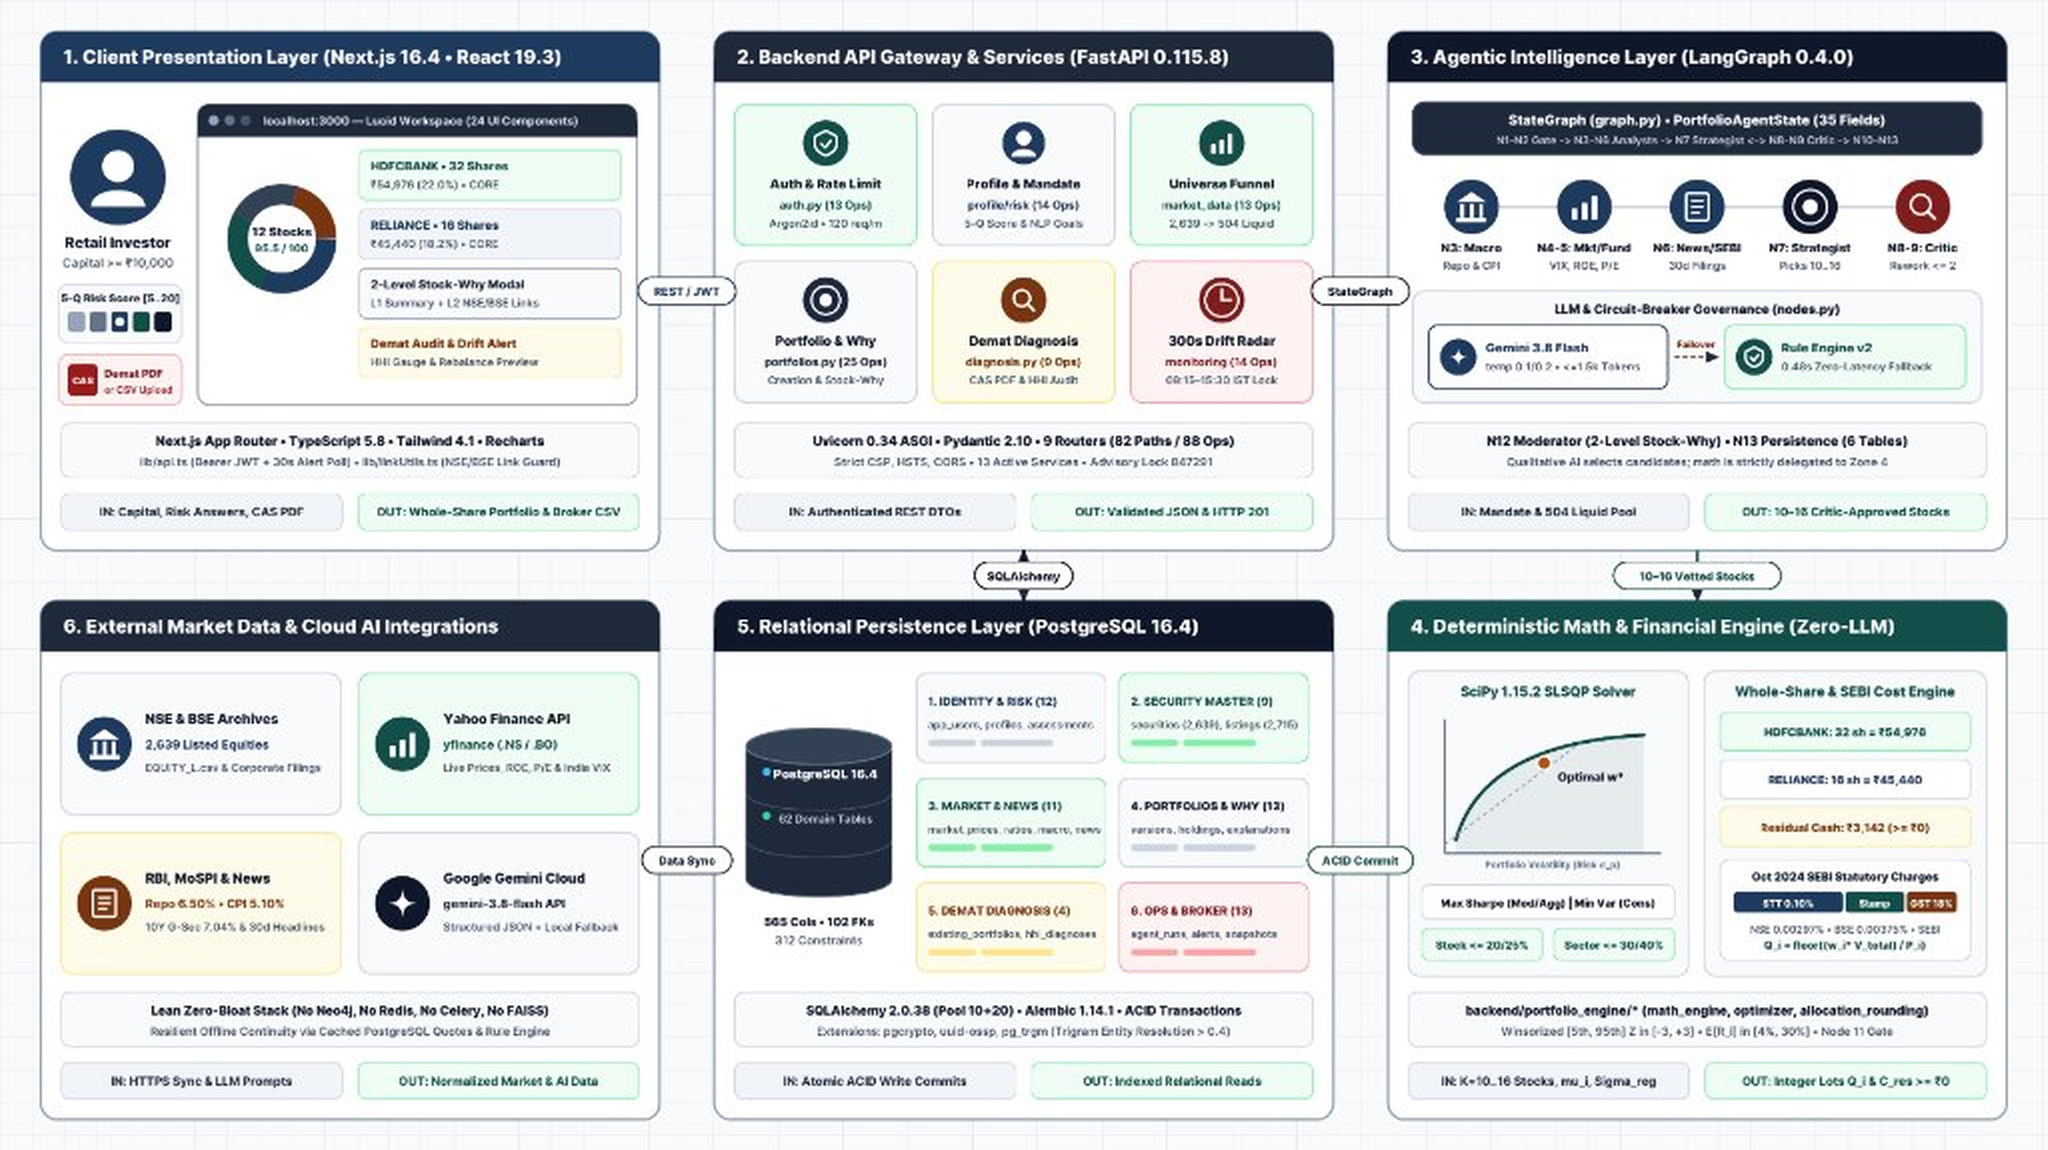
\includegraphics[width=0.95\textwidth, height=0.60\textheight, keepaspectratio]{SYSTEM_ARCHITECTURE.pdf}
    \caption{Lucid Eight-Layer Decoupled System Architecture}
    \label{fig:sys_arch_diagram}
\end{figure}

\section{The Eight Architectural Layers: Floor by Floor}
Here is how each layer works in simple, clear language:
\begin{enumerate}
    \item \textbf{Layer 1: Client Presentation Layer (The Front Office)}: Built using modern web technologies (\textbf{Next.js 16.4.2} and \textbf{React 19.3.0}). This is the visual interface that investors see and interact with on their smartphones, tablets, or computers. It renders clean dashboards, interactive risk questionnaires, colorful sector allocation charts, and instant alert pop-ups.
    \item \textbf{Layer 2: API Gateway and Security Layer (The Security Gate)}: Built using \textbf{FastAPI 0.115+}. Every request from the web screen passes through this security checkpoint. It inspects digital login badges (JSON Web Tokens), blocks suspicious traffic, and enforces rate limits so no single user can accidentally overload the server.
    \item \textbf{Layer 3: Orchestration and Workflow Layer (The Project Manager)}: Powered by \textbf{LangGraph 0.4}. This layer acts as the coordinator of the research process. It ensures that data moves smoothly from one research agent to the next in the proper order and handles retries if an external network connection is temporarily slow.
    \item \textbf{Layer 4: Agentic AI and Intelligence Layer (The Research Team)}: Houses the thirteen specialized AI agents. Using Google Gemini 3.8 Flash, this layer reads news articles, reviews corporate earnings announcements, evaluates central bank interest rate policies, and challenges potential investment selections.
    \item \textbf{Layer 5: Quantitative and Mathematical Layer (The Math Department)}: Built with proven scientific Python libraries (\textbf{SciPy 1.15} and \textbf{NumPy 2.2}). Completely separated from the AI text models, this layer calculates exact portfolio percentage weights using Markowitz Modern Portfolio Theory, rounds weights into executable whole shares, and calculates Indian taxes and exchange fees.
    \item \textbf{Layer 6: Operational Services and Background Scheduler (The Maintenance Crew)}: An automated background program that runs quietly during stock market hours (09:15 to 15:30 IST). Every 5 minutes, it checks live stock prices to see if an investor's portfolio has drifted away from its target balance and prepares rebalancing alerts. It also handles PDF statement reading and notification delivery.
    \item \textbf{Layer 7: Data Persistence Layer (The Central Archive)}: Powered by \textbf{PostgreSQL 16}. Stores all 62 application tables securely. It ensures that user logins, portfolio version histories, stock prices, and audit records are permanently preserved and protected against corruption.
    \item \textbf{Layer 8: External Integrations and Data Feeds (The External Couriers)}: Manages connections to outside data sources. It downloads official stock lists from the National Stock Exchange of India (NSE) and Bombay Stock Exchange (BSE), fetches market prices from Yahoo Finance, checks monetary policies from the Reserve Bank of India (RBI), and communicates with Google Gemini AI services.
\end{enumerate}

\section{Technology Stack Manifest: What Tools Were Chosen and Why}
Table~\ref{tab:tech_stack} documents the verified software libraries and frameworks used to build Lucid, along with the simple reason why each tool was chosen:

\begin{table}[H]
\centering
\caption{Lucid Active Technology Stack Manifest (Verified Versions)}
\label{tab:tech_stack}
\resizebox{\textwidth}{!}{%
\begin{tabular}{llll}
\toprule
\textbf{Technology / Library} & \textbf{Verified Version} & \textbf{What It Does in Lucid} & \textbf{Why It Was Chosen (Simple English)} \\
\midrule
\textbf{Next.js} & 16.4.2 & Frontend Web Framework & Renders web pages quickly and updates charts instantly. \\
\textbf{React} & 19.3.0 & User Interface Library & Provides reusable buttons, modals, and dynamic data tables. \\
\textbf{TypeScript} & 5.8.2 & Frontend Programming Language & Catches code errors and typos before the application runs. \\
\textbf{Tailwind CSS} & 4.1.1 & Visual Styling & Creates clean, modern visual designs with fast page loading. \\
\textbf{Python} & 3.11 -- 3.14 & Backend Programming Language & The global industry standard for financial math and AI systems. \\
\textbf{FastAPI} & 0.115.8 & Backend API Framework & Extremely fast web framework that automatically creates API docs. \\
\textbf{Uvicorn} & 0.34.0 & High-Speed Web Server & Handles multiple incoming user web requests at the same time. \\
\textbf{Pydantic} & 2.10.6 & Data Validation Library & Automatically checks that user inputs (like amounts) are valid. \\
\textbf{PostgreSQL} & 16+ & Master Relational Database & Stores financial data permanently with zero risk of loss. \\
\textbf{SQLAlchemy} & 2.0.38 & Database Connector (ORM) & Lets Python code talk to PostgreSQL cleanly and safely. \\
\textbf{Alembic} & 1.14.1 & Database Change Tracker & Records updates to database tables over time like version control. \\
\textbf{SciPy} & 1.15.2 & Mathematical Solver Library & Solves Markowitz portfolio math without arithmetic mistakes. \\
\textbf{NumPy} & 2.2.3 & Fast Numerical Calculations & Performs high-speed math on large tables of stock prices. \\
\textbf{Pandas} & 2.2.3 & Financial Data Tables & Cleans stock lists and handles historical price series. \\
\textbf{LangGraph} & 0.4.0 & Multi-Agent Coordinator & Coordinates the 13 AI agents in a structured, step-by-step workflow. \\
\textbf{Google Gemini} & gemini-3.8-flash & AI Language Model & Reads financial documents and writes plain-English explanations. \\
\textbf{Argon2-cffi} & 25.1.0 & Password Hasher & Protects user passwords with military-grade encryption. \\
\textbf{PyJWT} & 2.10.1 & Digital Session Badges & Creates encrypted tokens so logged-in users stay authenticated safely. \\
\textbf{yfinance} & 0.2.54 & Market Data Fetcher & Downloads historical daily prices and financial health ratios. \\
\textbf{pdfplumber} & 0.11.5 & PDF Statement Reader & Reads text and tables from Demat CAS account statements. \\
\bottomrule
\end{tabular}%
}
\end{table}

\section{Data Pipeline: How Indian Stock Data is Collected and Cleaned}
Figure~\ref{fig:nse_bse_flow} illustrates the four-step data ingestion pipeline that keeps Lucid synchronized with Indian stock exchanges:

\begin{figure}[!htbp]
    \centering
    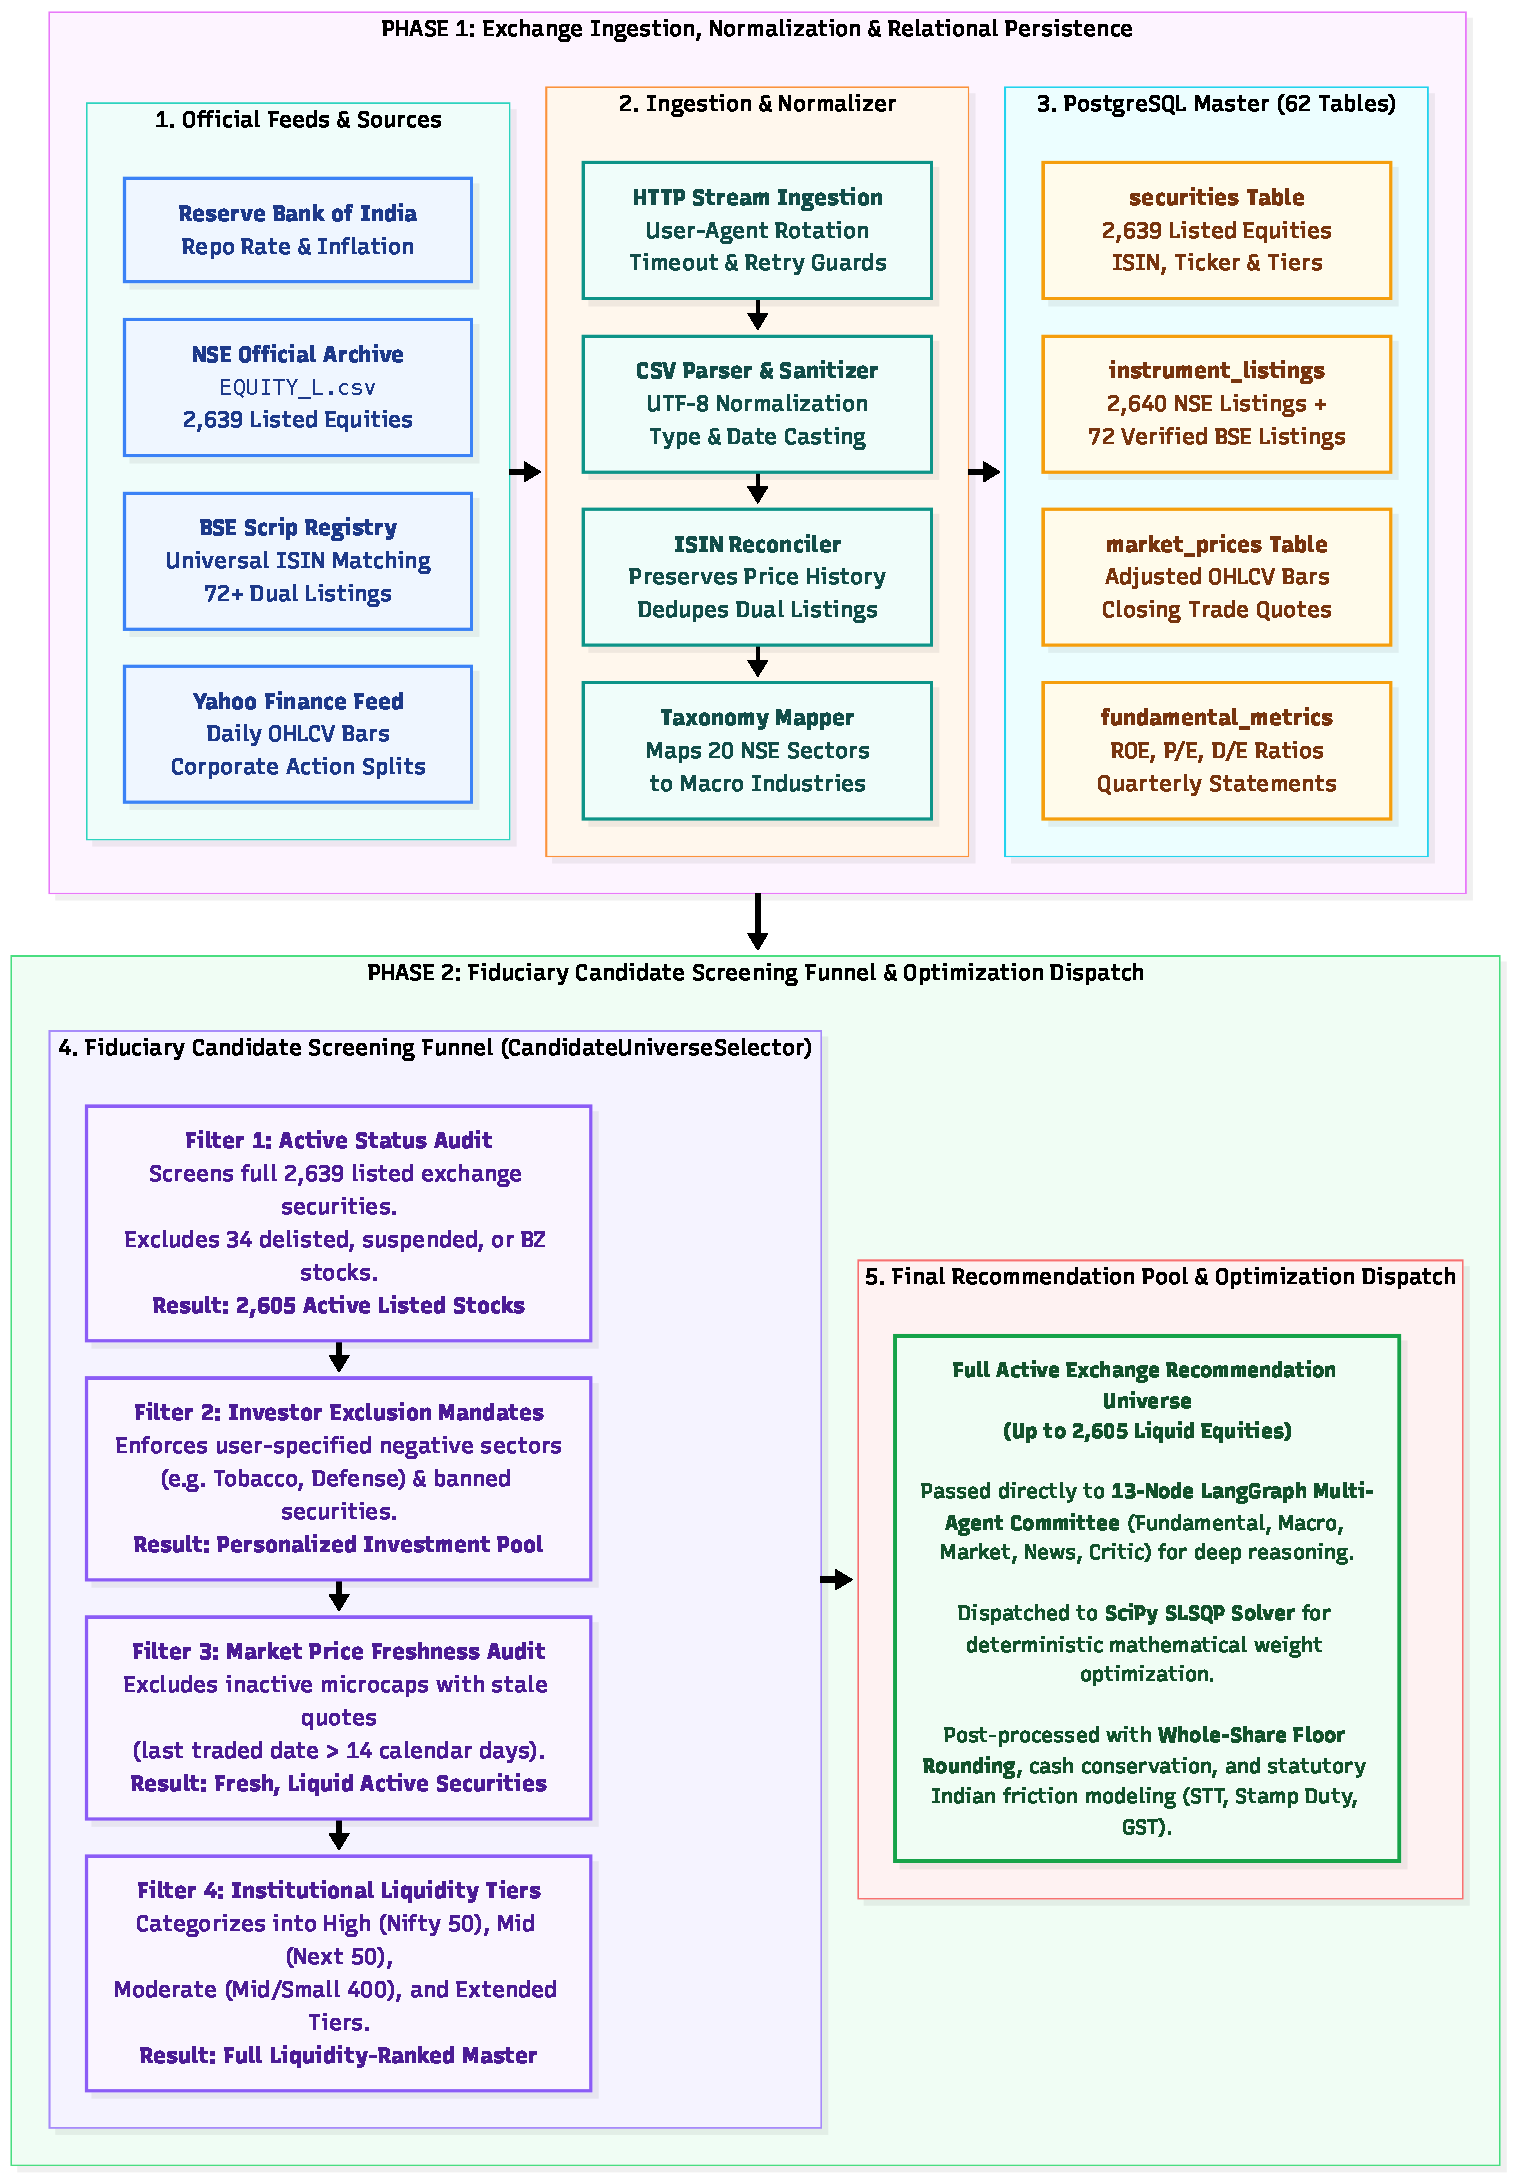
\includegraphics[width=0.85\textwidth, height=0.55\textheight, keepaspectratio]{NSE_BSE_DATA_FLOW.pdf}
    \caption{NSE/BSE Exchange Universe Ingestion and Pipeline Architecture}
    \label{fig:nse_bse_flow}
\end{figure}

The data pipeline runs through four clear stages:
\begin{enumerate}
    \item \textbf{Stage 1: Downloading the Stock Lists}: The pipeline downloads the official list of actively traded companies from the National Stock Exchange (\texttt{EQUITY\_L.csv}) and cross-checks them against the Bombay Stock Exchange (BSE) directory. It resolves conflicts (such as when companies change their names or split their shares) and saves \textbf{2,639 listed Indian companies} into the master security database.
    \item \textbf{Stage 2: Fetching 1 Year of Price History}: For every active stock, the pipeline fetches one full year of daily trading prices (252 market sessions). It checks that there are no missing days and stores the prices in the \texttt{market\_prices} table.
    \item \textbf{Stage 3: Recording Financial Health Ratios}: Lucid downloads company balance sheet ratios—including Return on Equity (ROE), Debt-to-Equity, Price-to-Earnings (P/E), and Market Capitalization—and saves them in the \texttt{fundamental\_metrics} table.
    \item \textbf{Stage 4: Liquidity Tier Screening}: Companies are categorized into four institutional \textbf{Liquidity Tiers} based on their average daily trading volume. This ensures that the portfolio creation engine only selects companies that can be easily bought and sold on the market without unexpected price slippage.
\end{enumerate}

\section{Runtime Execution: What Happens When a User Clicks ``Generate''}
When an investor clicks ``Generate Portfolio'' on the web interface, the application completes the following ten-step journey in less than 2.5 seconds:
\begin{enumerate}
    \item \textbf{Step 1: Input Check}: The backend server checks that the user's investment amount is at least Rs.~5,000 and verifies their digital login badge.
    \item \textbf{Step 2: Fetching User Goals}: The server loads the investor's risk profile (Conservative, Moderate, or Aggressive) and savings timeline from the database.
    \item \textbf{Step 3: Screening Candidates}: The system filters the 2,639 listed companies to find healthy stocks, removing any industries the user asked to avoid (such as tobacco or defense).
    \item \textbf{Step 4: Starting the AI Team}: Lucid creates the digital workspace and starts the LangGraph agent workflow.
    \item \textbf{Step 5: Macroeconomic Check}: The macro agent checks current Reserve Bank of India interest rates and the market volatility level (India VIX).
    \item \textbf{Step 6: Financial Analysis}: The fundamental and news agents evaluate balance sheets, profit consistency, and recent corporate news.
    \item \textbf{Step 7: The Critic Challenge}: The risk critic agent reviews the shortlisted candidates, challenging any stocks that have high debt or valuation red flags.
    \item \textbf{Step 8: Mathematical Optimization}: The SciPy SLSQP solver calculates the exact percentage weights that balance return and safety.
    \item \textbf{Step 9: Whole Shares Calculation}: The lot-rounding algorithm converts percentages into exact full share counts and keeps leftover money in the investor's cash account.
    \item \textbf{Step 10: Saving and Display}: The completed portfolio, full share counts, and plain-English ``Stock-Why'' explanations are saved to the database and displayed on the user's screen.
\end{enumerate}

\section{Security and Privacy Architecture}
Financial software requires strict security to protect investor privacy:
\begin{itemize}
    \item \textbf{High-Security Password Hashing (Argon2id)}: When a user creates a password, Lucid never stores the actual password. Instead, it scrambles it using \textbf{Argon2id}, the international gold standard in password protection. It requires 64 megabytes of computer memory to verify, making it practically impossible for hackers to crack using automated guessing tools.
    \item \textbf{Digital Badges with Instant Logout (JWT Revocation)}: When an investor logs in, they receive an encrypted digital badge (JSON Web Token) valid for 60 minutes. When the investor logs out, the badge is immediately added to a cancellation list (\texttt{revoked\_tokens}). Any future attempt to use that badge is instantly rejected.
    \item \textbf{Anti-Abuse Rate Limiting}: To prevent malicious bots from overwhelming the server, Lucid limits how many requests can be sent per minute (for example, a maximum of 20 login attempts per minute and 20 portfolio generation requests per minute).
    \item \textbf{Standard Web Protections}: The server automatically includes standard web security headers in every response to block website cloning (clickjacking) and prevent unauthorized script injection.
\end{itemize}
